% !TEX encoding = UTF-8
% !TEX TS-program = pdflatex
% !TEX root = ../tesi.tex

%**************************************************************
\chapter{Il contesto aziendale}
\label{cap:contesto_aziendale}
%**************************************************************
\section{Profilo aziendale}
Crispy Bacon srl\footnote{Crispy Bacon srl. URL: \href{https://crispybacon.it/}{https://crispybacon.it}} è una software development company nata nel 2013 da quattro soci fondatori e che conta oggi più di 50 persone tra le sedi di Marostica (VI) e Milano. Una realtà "technology driven" (dipendere dalla tecnologia e utilizzarla in modo pratico), volta a cogliere le migliori tecnologie presenti sul mercato per offrire ai clienti strumenti digitali sempre più avanzati e innovativi, ne sono un recente esempio le applicazioni per smart speakers quali Amazon Alexa\footnote{Amazon Alexa. URL: \href{https://developer.amazon.com/it/alexa}{https://developer.amazon.com/it/alexa}} e Google Home.\\
L’obiettivo di Crispy Bacon è quello di entrare nel mercato italiano con tecnologie di frontiera quali soluzioni bancarie, per l'industria e la moda.
I principali servizi offerti rientrano nel campo dello sviluppo web e mobile, consulenza nell'ambito della digital transformation, UX/UI design e cloud computing, sempre al fianco dei propri clienti.
Quello che Crispy Bacon si prefigge è di realizzare esperienze soddisfacenti mediante l’utilizzo di metodologie, approcci e tecnologie dirompenti.
\begin{figure}[H] 
    \centering 
    
\includegraphics[width=0.7\columnwidth]{immagini/logo.png}
    \caption{\label{fig:logo_cripsy}Logo Crispy Bacon srl}
\end{figure}
%**************************************************************
\section{Dominio applicativo}
\subsection{Alexa}
Alexa\footnote{\href{Alexa. URL: https://it.wikipedia.org/wiki/Amazon\_Alexa}{https://it.wikipedia.org/wiki/Amazon\_Alexa}} è un assistente vocale intelligente basato su computabilità cloud sviluppato dalla sezione Lab126\footnote{Società americana di ricerca e sviluppo hardware per computer.} di Amazon utilizzato sui dispositivi in commercio quali Amazon Echo ed Echo Dot. Con Alexa, è possibile sviluppare performance vocali naturali che offrono ai clienti un modo più intuitivo per interagire con la tecnologia che utilizzano tutti i giorni. È in grado quindi di interpretare il linguaggio naturale e dialogare fornendo informazioni di diverso tipo. Le funzioni più comuni sono: riprodurre musica, gestire liste (della spesa o delle cose da fare), impostare promemoria e sveglie, effettuare streaming di brani musicali e podcast, riprodurre audiolibri e fornire previsioni meteorologiche, informazioni sul traffico e riprodurre altre informazioni in tempo reale, come le notizie. Alexa é in grado anche di controllare diversi dispositivi intelligenti, usando se stesso come sistema di automazione domestica per la gestione della domotica.

\subsection{Skill}
Come detto in precedenza, alcune funzioni di Alexa sono native, quali ricerche sul web, sveglie, liste, meteo, ecc.. Alexa fornisce inoltre delle Skill, ovvero dell'applicazioni di terze parti appositamente sviluppate in base alle necessità, che consentono di creare un’esperienza d'uso più personalizzata.
Tali Skill possono essere installate nel proprio dispositivo su cui risiede l'assistente vocale ed avviate utilizzato il comando di lancio.
Amazon mette quindi a disposizione molteplici servizi dedicati, tra cui la vendita all'interno dello store, per creare Skill in modo da rendere l'esperienza di utilizzo personale unica.

\subsection{Amazon Web Service}
Amazon Web Services Inc, nota ed abbreviata con la sigla AWS, è un'azienda di proprietà di Amazon che fornisce più di 165 servizi completi di cloud computing\footnote{Servizi on-demand da un fornitore ad un cliente finale attraverso la rete Internet} tra cui data center, email service e moltro altro. Questi servizi offerti sono operativi in 20 paesi sparsi in tutto il mondo, a breve anche in Italia, che conta di arrivare a 24 aree geografiche entro il 2020. AWS offre molti servizi utilizzati per la realizzazione di questo progetto, tra i quali Amazon Lambda, DynamoDB e Amazon Simple Storage Service (S3), fornendo quindi soluzioni on-demand con caratteristiche di high availability\footnote{Caratteristica di un sistema, che mira a garantire un livello concordato di prestazioni operative per un periodo superiore al normale.}, ridondanza e sicurezza. Tali servizi possiedono combinazioni tra costo finale, caratteristiche, tempo di utilizzo e performances ottimali per utenti e le aziende. Tali caratteristiche rendono l'ecosistema di AWS grande e dinamico, con milioni di clienti attivi, di ogni settore e dimensione, incluse start-up, aziende e organizzazioni del settore pubblico in tutto il mondo.
\begin{figure}[H] 
    \centering 
    
\includegraphics[width=0.8\columnwidth]{immagini/alexa_awspng.png}
    \caption{\label{fig:alexa_aws}Logo di Alexa e AWS}
\end{figure}

\subsection{L'idea}
Nasce da qui l'idea di voler realizzare, sfruttando l'ecosistema di AWS e l'assistente vocale Alexa, un concierge virtuale che possa, in maniera facile e pratica, accogliere clienti e visitatori senza l'intervento umano in maniera totalmente automatica.

\subsection{Interesse aziendale}
L'azienda desidera la sua realizzazione per uso personale all'interno degli uffici e come prototipo per poter sviluppare prodotti simili al fine di proporli ai clienti in maniera personalizzata o preconfezionata.

\subsection{Il progetto}
Nasce da questa idea il progetto Concierge Croccante, una Skill da poter installare sugli speakers Amazon con integrato l'assistente vocale Alexa. Essa permetterà di annunciarsi ed essere accolti al momento dell'ingresso presso un ufficio, innescando un processo di accettazione e di notifica agli interessati dell'arrivo dell'ospite.

\section{Metodologia aziendale}
Cripsy Bacon è da considerarsi un'azienda di medio/piccole dimensioni, di giovane età, in veloce espansione ed inserimento nel mercato digitale attraverso le sue numerose soluzioni home banking realizzate. Il progetto sviluppato e, in un futuro venduto, è caratterizzato da dimensioni e costi contenuti. Da tali informazioni si deduce che: 
\begin{itemize}
    \item il periodo di tirocinio, quindi il tempo dedicato al progetto, e le dimensioni medio/piccole, con la relativa giovinezza dell'azienda, comportino a prendere scelte rapide e sicure sull'uso delle tecnologie cosi da prediligere l'implementazione rapida di uno o più prototipi su cui sviluppare il prodotto finale;
    \item le tendenze tecnologiche del mercato sono fortemente dinamiche, necessitando così l'esigenza da parte dell'azienda nel volersi proporre con idee nuove ed innovative.
\end{itemize}
\begin{figure}[H] 
    \centering 
    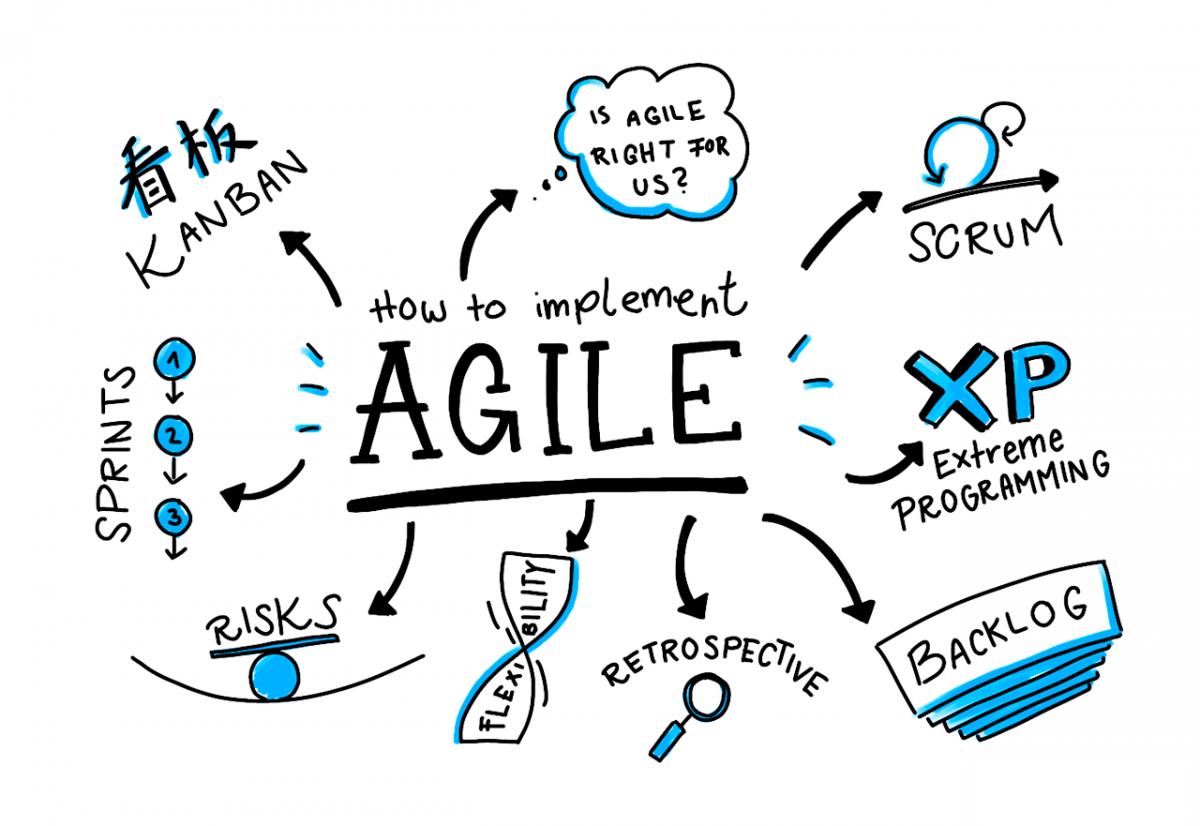
\includegraphics[width=1\columnwidth]{immagini/scrum.png}
    \caption{\label{fig:alexa_aws}Modello Agile - SCRUM}
\end{figure}
Sulla base di tali considerazioni, in accordo con l'azienda, la scelta sulla metodologia di sviluppo è ricaduta sul modello di lavoro agile\footnote{\href{Modello agile: URL: https://agilemanifesto.org/iso/it/manifesto.html}{https://agilemanifesto.org/iso/it/manifesto.html}} utilizzando il framework Scrum\footnote{Framework Scrum. URL: \href{https://it.wikipedia.org/wiki/Scrum\_(informatica)}{https://it.wikipedia.org/wiki/Scrum\_(informatica)}}. Tale framework viene adattato dell'azienda nel seguente modo:
\begin{itemize}
    \item Team di sviluppo: ogni progetto viene assegnato a più macro-team di sviluppo, composto mediamente da cinque o sei persone, come per esempio esiste il team per lo sviluppo del backend, per la realizzazione del frontend ed altro. Nel caso del progetto Consierge Croccante è stato organizzato un micro-team di due persone per il backend e una sola persona del reparto grafica per il frontend;
    
    \item Sviluppo per incremento: l’azienda Crispy Bacon adotta appieno questo approccio di sviluppo, creando di volta in volta liste di funzionalità da implementare per l'incremento successivo;
    
    \item Scrum: la riunione che rappresenta lo Scrum viene effettuata ogni tre giorni dal micro-team che si occupa del backend, in presenza del CFO e fondatore Damiano Buscemi;
    
    \item ScrumMaster: all'interno del micro-team il tutor aziendale ha ricoperto il ruolo di ScrumMaster;
    
    \item Sprint: il concetto di sprint definito nel framework Scrum viene applicato ed eseguito appieno dall'azienda. Uno sprint è stato disposto per la durata di circa due settimane;
    
\end{itemize}

\section{Tecnologie utilizzate}
\subsection{Node.js}
\label{nodejs}
Per la realizzazione del codice è stato scelto di utilizzare come linguaggio Node.js, una runtime multipiattaforma orientato agli eventi per l'esecuzione di codice JavaScript Server-side. Tale scelta è motivata dal fatto che i servizi implementati offrono API e pacchetti per questo linguaggio. Node.js consente di utilizzare JavaScript per scrivere codice da eseguire lato server, questo permette quindi di eseguire il codice sui servizi cloud computing quali Amazon Lambda. Altra particolarità di NodeJs la sua architettura orientata agli eventi che rende possibile l’inserimento di input/outputn asincrono. 

\subsection{Alexa Presentation Language}
Come accennato il progetto è costituito da un'interfaccia grafica che servirà di supporto al compimento del dialogo con la Skill. Per ottenere ciò è stato scelto di utilizzate Alexa Presentation Language\footnote{Alexa Presentation Language. URL: \href{https://developer.amazon.com/it/docs/alexa-presentation-language/apl-overview.html}{https://developer.amazon.com/it/docs/alexa-presentation-language/apl-overview.html}} messo a disposizione da Amazon. Esso permette di sviluppare il software con esperienze vocali e visive utilizzando layout. Si ha pertanto la flessibilità di sviluppare Skill multimodali con elementi visivi, tra cui grafica, immagini e la personalizzazione di output per dispositivi diversi. Quando si progetta utilizzando Alexa Presentation Language, vengono creati dei documenti APL, ovvero file JSON inviati dalla Skill al dispositivo. Quest'ultimo elabora il documento APL, importa immagini e dati per poi mostrare il risultato.

\subsection{Servizi Amazon Web Service}
\label{serivizi_aws}
AWS offre un ecosistema popolato da numerosissimi servizi già connessi tra loro. La scelta quindi di utilizzare tale ecosistema risulta la più conveniente e la più ottimale. Pertanto nel progetto vengono utilizzati i seguenti servizi:
\begin{itemize}
    \item AWS IAM: per gestire la sicurezza e gli accesso ai servizi e risorse di AWS
    \item AWS Cloud Watch: per monitorare e osservare l'esecuzione delle funzioni
    \item AWS DynamoDB: per il servizio di database non relazionale 
    \item AWS Lambda: per eseguire codice senza dover effettuare il provisioning e gestire server
    \item AWS SES: per il servizio di invio mail 
    \item AWS S3: per il servizio di storage di oggetti 
\end{itemize}

\subsection{Google Calendar}
Obbiettivo importante del prodotto è quello di poter consultare un calendario dove vengono trascritti gli impegni, eventi e appuntamenti dell'azienda. La scelta è ricaduta su l'utilizzo di Google Calendar, già utilizzado da Crispy Bacon, ovvero un sistema di calendari realizzato da Google che offre la possibilità di creare più calendari, di condividerli e importarli da altri servizi online. Difatti, quest'ultima caratteristica, agevola il collegamento tra Skill e calendario grazie a pacchetti ed API documentate.

\subsection{Slack}
Per l'invio di notifiche la scelta ricade su Slack, uno strumento software che permette di inviare messaggi in modo istantaneo, già conosciuto ed utilizzato da Crispy Bacon. Tale softfware agevola il collegamento tra Skill e la notifica istantanea grazie ad API pubbliche e documentate.  

\begin{figure}[H] 
    \centering 
    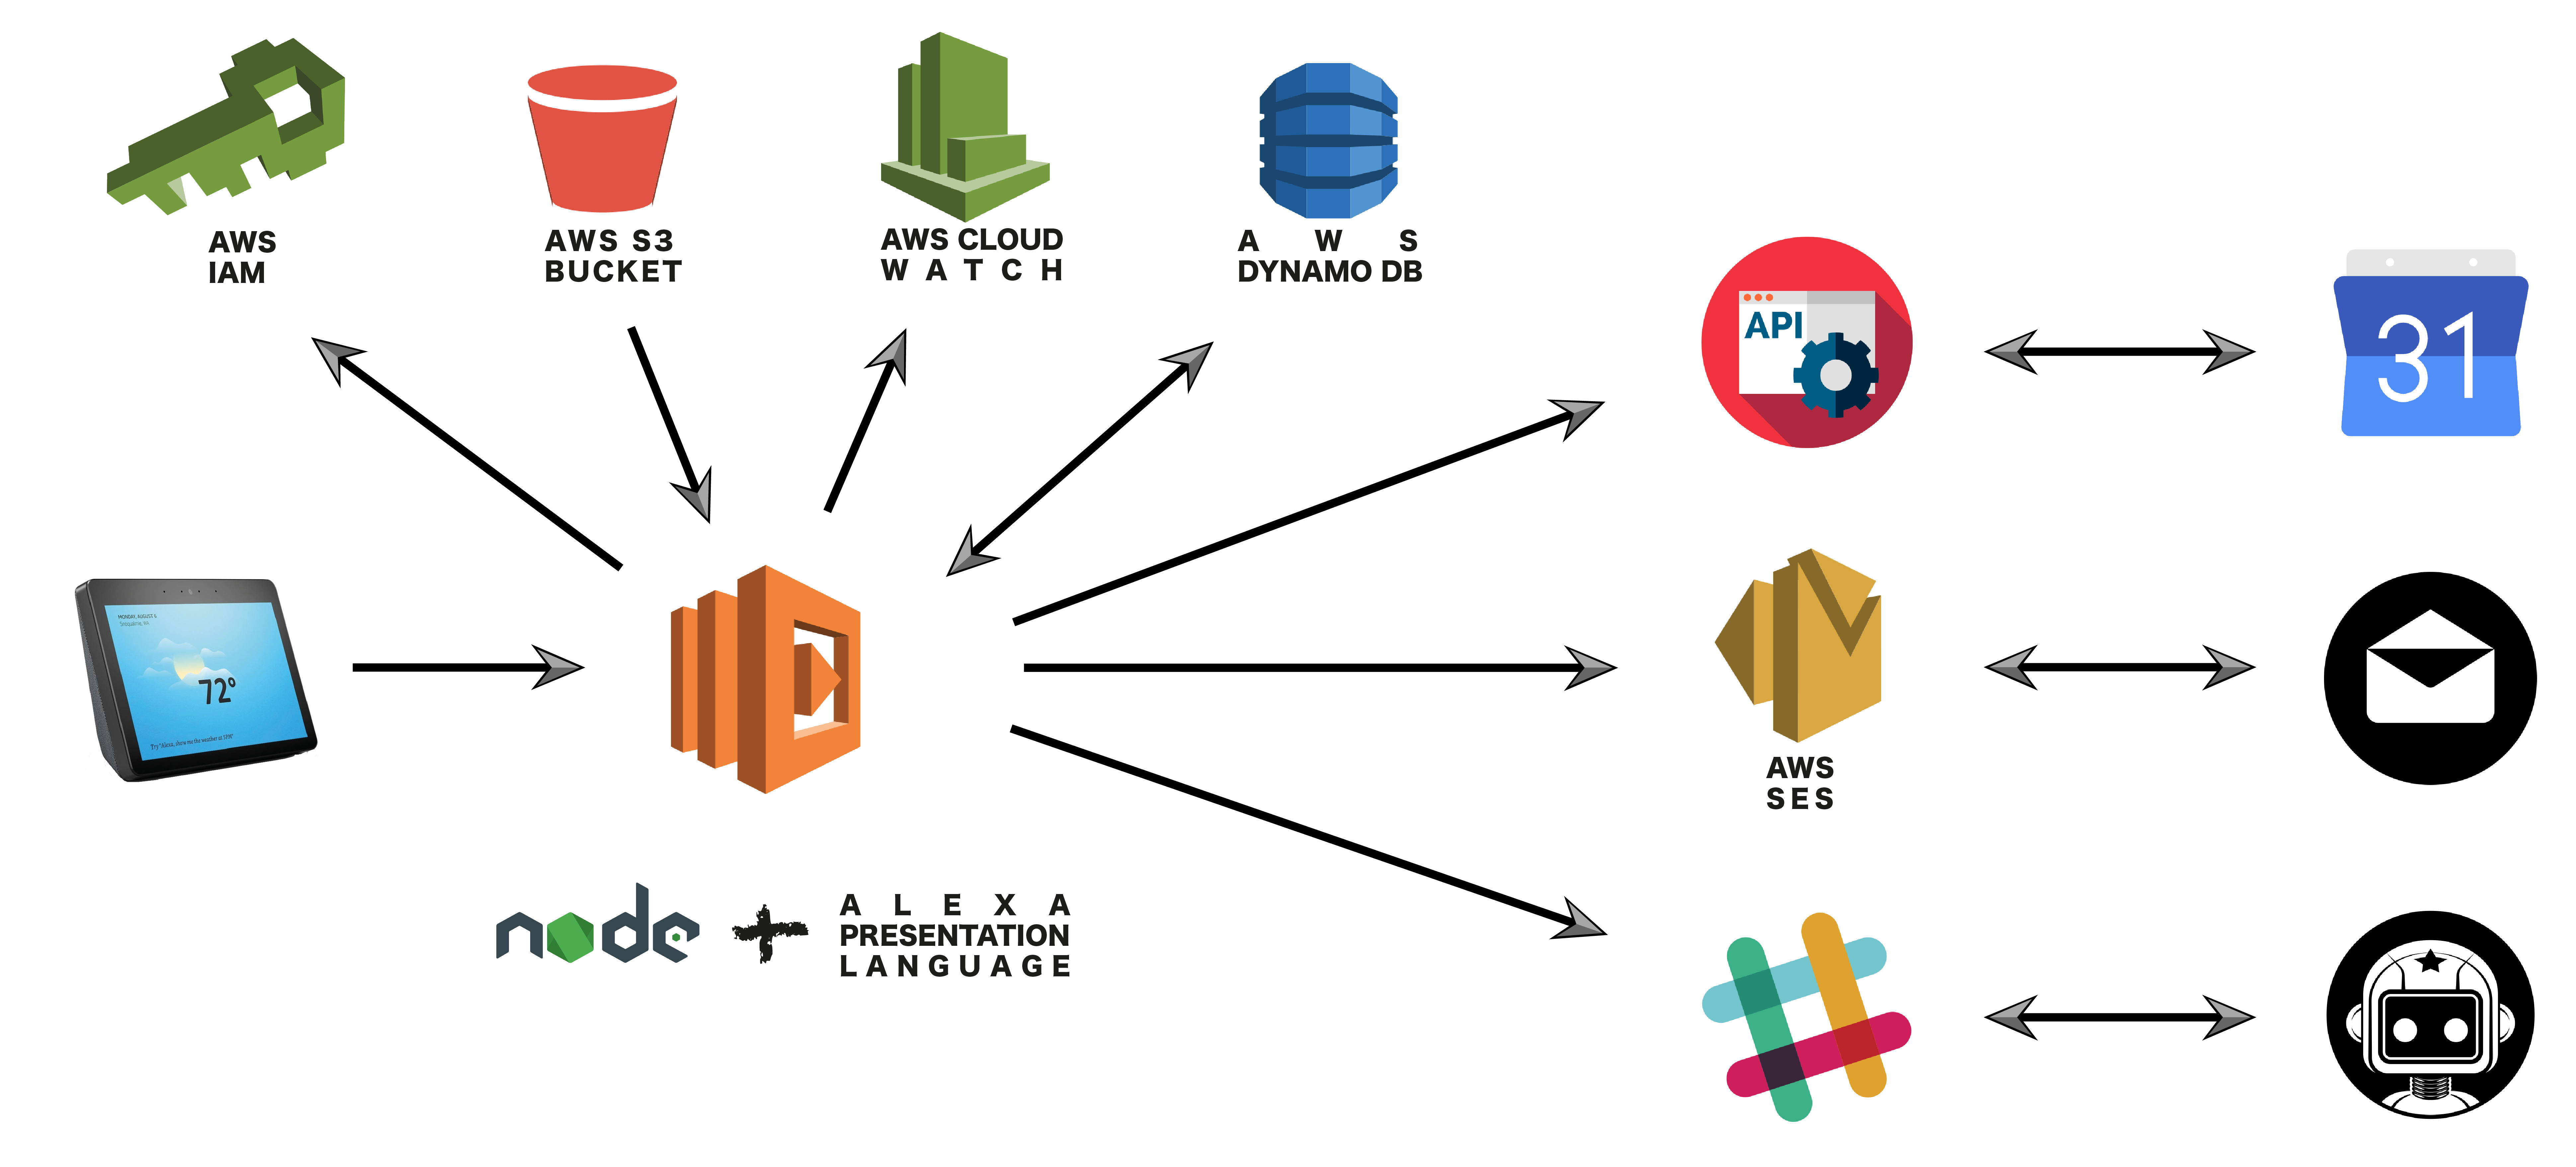
\includegraphics[width=1\columnwidth]{immagini/architettura.png}
    \caption{\label{fig:alexa_aws}Logo di Alexa e AWS}
\end{figure}

\section{Strumenti utilizzati}
\subsection{Alexa Developer Console}
Per realizzare la Skill è essenziale l'uso di Alexa Developer Console\footnote{Alexa Developer Console. URL: \href{https://developer.amazon.com/it/docs/devconsole/about-the-developer-console.html}{https://developer.amazon.com/it/docs/devconsole/about-the-developer-console.html}}, una console per gli sviluppatori che organizza lo sviluppo nelle seguenti attività principali:
\begin{itemize}
    \item Build: per realizzare e impostare la Skill creata, configurare il modello di interazione e specificare gli endpoint per il servizio.
    \item Test: per testare le Skill con l'assistente Alexa usando testo o voce.
    \item Distribuzione: per vedere in anteprima come appariranno le Skill nello store.
    \item Certificazione: per convalidare la Skill creata, eseguire test di pre-certificazione e infine inviare la Skill per la certificazione.
    \item Analytics: per rivedere le metriche relative alle Skill create.
\end{itemize}

\subsection{Amazon Echo Show}
Per vedere e testare il prodotto finale si è usato l'Amazon Echo Show, uno smart display da 10" che integra l’assistente vocale Amazon Alexa. Controllabile con la voce, è in grado di interagire con gli utenti, eseguire diversi comandi vocali oltre che mostrare i contenuti direttamente sullo schermo touch.

\subsection{NPM}
\label{npm}
Per installare i pacchetti necessari è stato utilizzato NPM, il principale software per gestire i moduli di Node.js e consente di condividere il codice per problemi tipici tra gli sviluppatori JavaScript. La filosofia alla base di tale gestore è quella che se un problema è stato già risolto da altri programmatori deve esser possibile utilizzare la soluzione condivisa messa a disposizione degli altri utenti. NPM oltre a consentire il riuso del codice, consente di tenerlo costantemente sotto controllo in modo da aggiornarlo. NPM suddivide inoltre il codice in package, ovvero una directory che contiene uno o più file insieme, dove un file chiamato package.json contiene i dati relativi al pacchetto.

\subsection{Gitlab}
Il versionamento degli applicativi viene fatto tramite Git\footnote{Git. URL: \href{https://git-scm.com/}{https://git-scm.com/}} e i repository sono ospitati su Gitlab\footnote{Gitlab. URL: \href{https://about.gitlab.com/}{https://about.gitlab.com/}} in un server dedicato dell'azienda. GitLab è una piattaforma che permette la gestione centralizzata dei repository Git, permettendo l'amministrazione dei permessi d'accesso tramite una semplice interfaccia grafica. Tutti gli applicativi e le configurazioni dell'infrastruttura vengono ospitati sulla piattaforma e il versionamento segue regole del Git-Flow dove le funzionalità nuove vengono sviluppate su un branch dedicato, per poi essere spostate successivamente nei branch di sviluppo, accettazione e infine produzione.

\subsection{Ambiente di sviluppo}
L’azienda non ha posto alcuna limitazione per quanto riguarda gli IDE lasciando libero arbitrio sulla scielta. Necessitando il progetto di diversi linguaggi quali Node.js e JSON la scelta è ricaduta su Visual Studio Code\footnote{Visual Studio Code. URL: \href{https://code.visualstudio.com/}{https://code.visualstudio.com/}}, IDE sviluppato da Microsoft\footnote{Microsoft. URL: \href{https://www.microsoft.com/}{https://www.microsoft.com/}} e consigliato per lavorare con progetti multi linguaggio, in quanto estensibile tramite plugin per supportare la maggior parte dei linguaggi di programmazione.
%**************************************************************
\section{Organizzazione del testo}
Il documento presenta la seguente struttura:
\begin{itemize}
    \item Capitolo 1: Introduzione comprende la descrizione generale dell'azienda ospitante e del relativo metodo di lavoro, una contestualizzazione ed illustrazione del progetto di stage ed infine la presentazione della struttura del documento
    \item Capitolo 2: Analisi dei Requisiti si tratta di una descrizione dettagliata della fase di analisi dei requisiti portata a termine dal candidato
    \item Capitolo ??
    \item Capitolo ??
    \item Capitolo ??
\end{itemize}




